\documentclass[12pt,t]{beamer}

\usepackage{graphicx}
\setbeameroption{hide notes}
\setbeamertemplate{note page}[plain]

% get rid of junk
\usetheme{default}
\beamertemplatenavigationsymbolsempty
\hypersetup{pdfpagemode=UseNone} % don't show bookmarks on initial view

% font
\usepackage{fontspec}
\setsansfont{TeX Gyre Heros}
\setbeamerfont{note page}{family*=pplx,size=\footnotesize} % Palatino for notes
% "TeX Gyre Heros can be used as a replacement for Helvetica"
% In Unix, unzip the following into ~/.fonts
% In Mac, unzip it, double-click the .otf files, and install using "FontBook"
%   http://www.gust.org.pl/projects/e-foundry/tex-gyre/heros/qhv2.004otf.zip

% named colors
\definecolor{offwhite}{RGB}{249,242,215}
\definecolor{foreground}{RGB}{255,255,255}
\definecolor{background}{RGB}{24,24,24}
\definecolor{title}{RGB}{107,174,214}
\definecolor{gray}{RGB}{155,155,155}
%\definecolor{darkgray}{RGB}{30,30,30}
\definecolor{subtitle}{RGB}{102,255,204}
\definecolor{hilight}{RGB}{102,255,204}
\definecolor{vhilight}{RGB}{255,111,207}
\definecolor{lolight}{RGB}{155,155,155}
\definecolor{green}{RGB}{125,250,125}

% use those colors
\setbeamercolor{titlelike}{fg=title}
\setbeamercolor{subtitle}{fg=subtitle}
\setbeamercolor{institute}{fg=gray}
\setbeamercolor{normal text}{fg=foreground,bg=background}
\setbeamercolor{item}{fg=foreground} % color of bullets
\setbeamercolor{subitem}{fg=gray}
\setbeamercolor{itemize/enumerate subbody}{fg=gray}
\setbeamertemplate{itemize subitem}{{\textendash}}
\setbeamerfont{itemize/enumerate subbody}{size=\footnotesize}
\setbeamerfont{itemize/enumerate subitem}{size=\footnotesize}

% page number
\setbeamertemplate{footline}{%
    \raisebox{5pt}{\makebox[\paperwidth]{\hfill\makebox[20pt]{\color{gray}
          \scriptsize\insertframenumber}}}\hspace*{5pt}}

% add a bit of space at the top of the notes page
\addtobeamertemplate{note page}{\setlength{\parskip}{12pt}}

% a few macros
\newcommand{\ig}{\includegraphics}
\newcommand{\subt}[1]{{\footnotesize \color{subtitle} {#1}}}

\usepackage{listings}

\lstset{language=bash,
        basicstyle=\tiny,
        frame=single,
        backgroundcolor=\color{darkgray},
        commentstyle=\color{green},
        foregroundcolor=\color{white}
        showstringspaces=false
        }

\newcommand{\ft}[1]{\frametitle{#1}}
\newcommand{\bi}{\begin{itemize}}
\newcommand{\bbi}{\vspace{24pt} \begin{itemize} \itemsep8pt}
\newcommand{\ei}{\end{itemize}}
\newcommand{\figw}[2]{\centerline{\includegraphics[width=#2\textwidth]{#1}}}
\newcommand{\figh}[2]{\centerline{\includegraphics[height=#2\textheight]{#1}}}
\newcommand{\fig}[1]{\centerline{\includegraphics{#1}}}

\title[git \& GitHub]{A brief introduction to git \& GitHub}
\author[Younkin \& Broman]{Samuel G. Younkin, Karl Broman}
\institute{Biostatistics \& Medical Informatics \\ University of Wisconsin{\textendash}Madison}
\date{\href{https://github.com/syounkin/GitPrimer}{\tt \scriptsize github.com/syounkin/GitPrimer}}

\begin{document}
\frame{\titlepage}

\frame{
\vspace*{12pt}

% comic from http://www.phdcomics.com/comics/archive.php?comicid=1531
\centerline{
\includegraphics[height=3.2in]{phd101212s.png}}
}

\section{Version control}
\frame{
\ft{\only<1>{Methods for tracking versions}\only<2>{Suppose it stops working\dots}}
\bbi
\item Don't keep track
\onslide<2>{
\bi
\item good luck!
\ei
}
\item Save numbered zip files
\onslide<2>{
\bi
\item Unzip versions and {\tt diff}?!
\ei
}
\item Formal version control
\onslide<2>{
\bi
\item Easy to study changes back in time
\item Easy to jump back and test
\ei
}
\ei
}

\frame{
\ft{Why use formal version control?}
\bbi
\item History of changes
\item Able to go back
\item No worries about breaking things that work
\item Merging changes from multiple people
\ei
}

\section{git}

\frame{
\ft{What is git?}
\bbi
\item Formal version control system
\item Developed by Linus Torvalds
\item Content Tracking System
\bi
\item Useful for reports, manuscripts, websites, as well as
  software
\ei
\ei
}

\frame{
\ft{Why is it named git?}
\bbi
\item git: British slang for a foolish or worthless person
\item Linus named the software after himself again
\item Hilarious yes, but perhaps not the best name for such a
  ubiquitous and powerful program \ei }

\frame{
\ft{Why use git (vs, say, subversion)?}
\bbi
\item It's fast
\item You don't need access to a server
\item Everyone's using it
\ei
}

\section{git Demo}

\begin{frame}[fragile]
\frametitle{Collaboration}
\bi
\item Sam \& Karl are collaborating on a presentation
\item They want:
\bi
%\item Two versions (CK Group \& Faculty)
\item Tracking ability
\bi\item Who made what change and when\ei
\item Backups need to be in place
\bi\item If Sam makes a mistake we must be able to undo it
\item If Karl changes his mind about the direction the project has taken we must be able to revert to any prior state
\ei
\item Publicly available
\bi\item So all may benefit from our insight\ei
\item Annotate changes
\bi\item If Sam makes a change it should be annotated formally so both Karl and future Sam know why it was made\ei
\ei
\item Not surprisingly, git and GitHub together satisfy all of these requirements
\ei
\end{frame}

\begin{frame}
\frametitle{A github repository}

\vfill
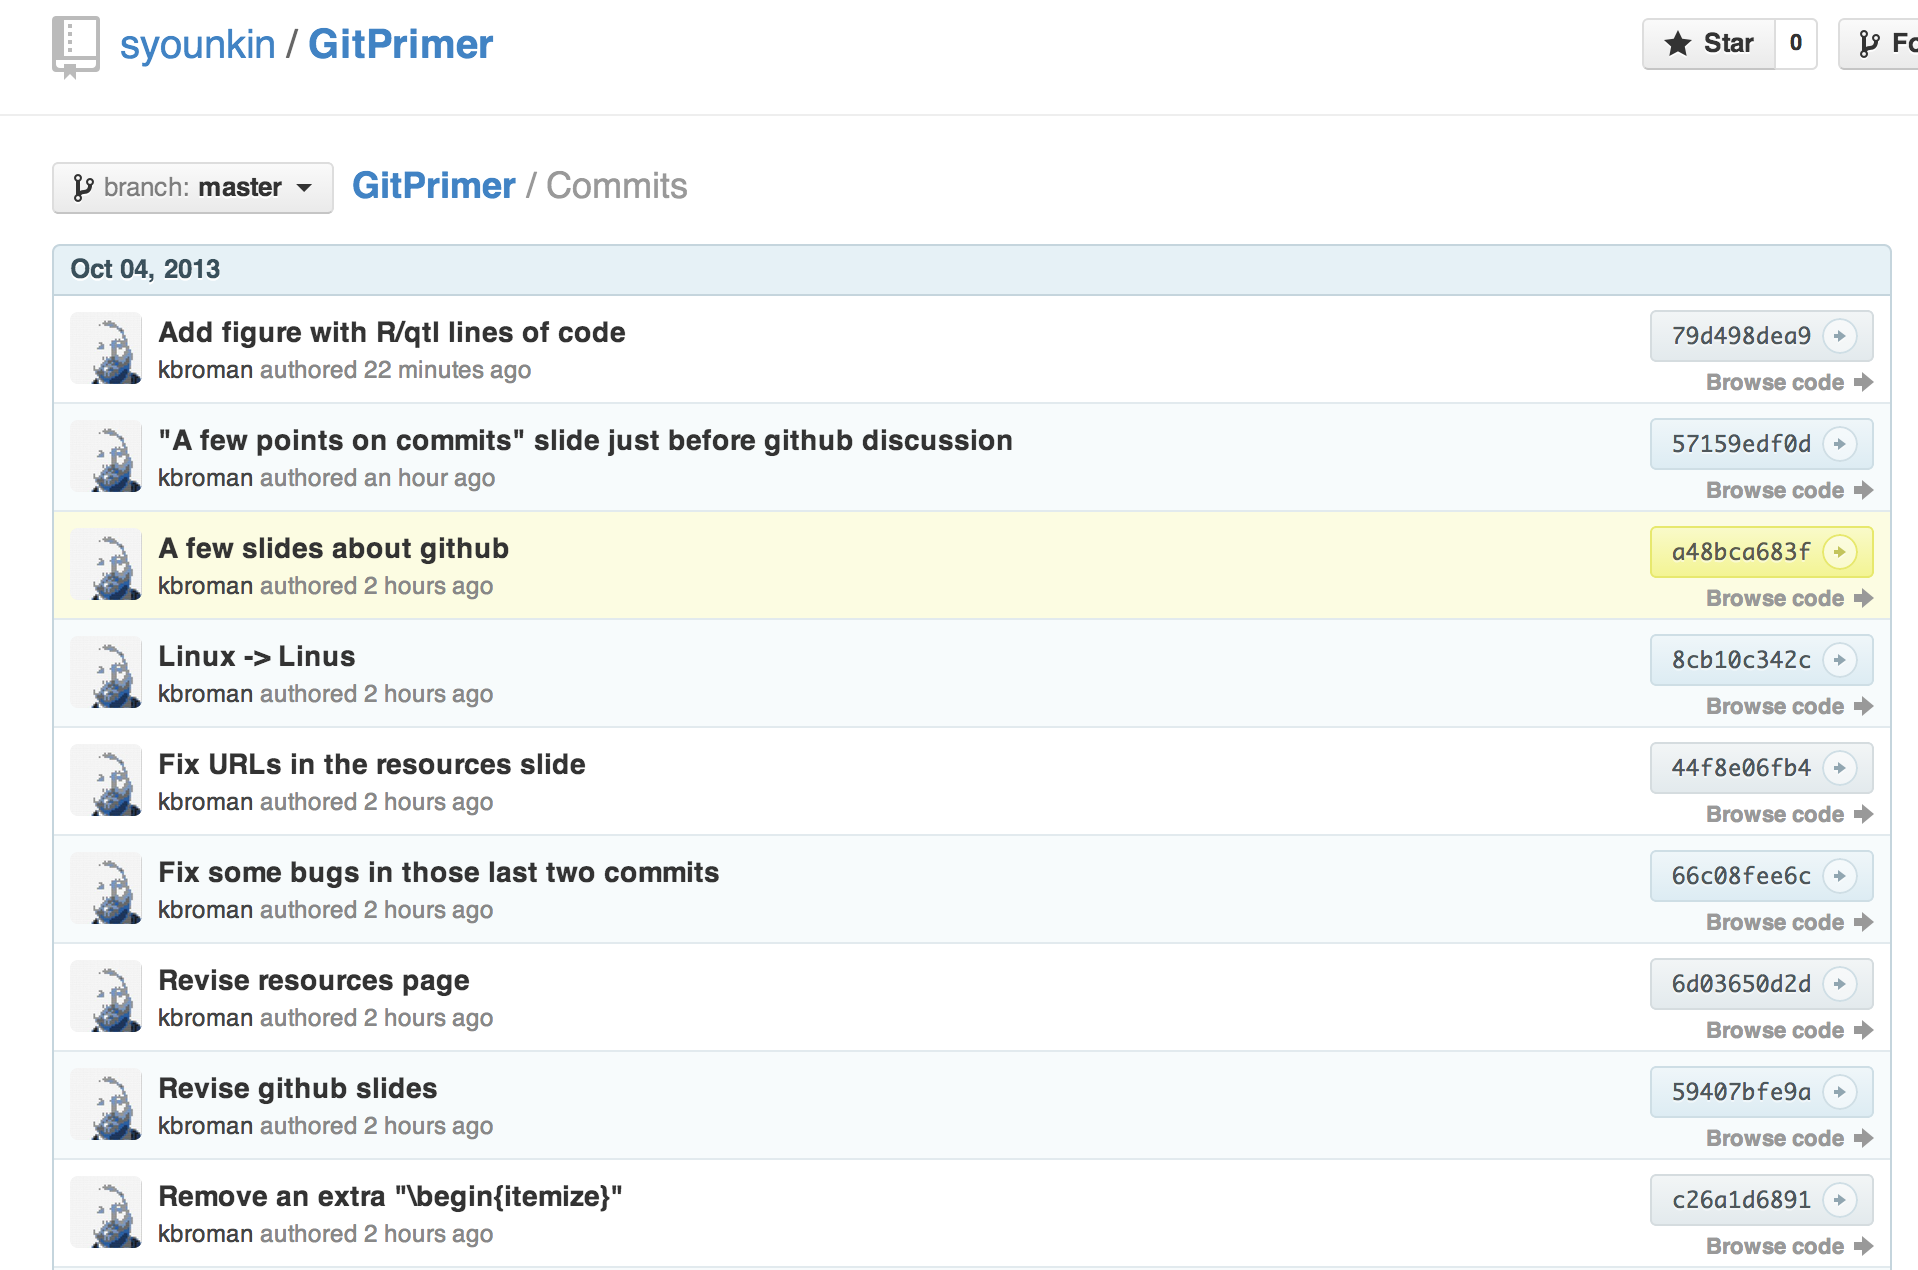
\includegraphics[height=2.2in]{list_of_commits.png}
\end{frame}

\begin{frame}
\frametitle{Details of a commit}

\vfill
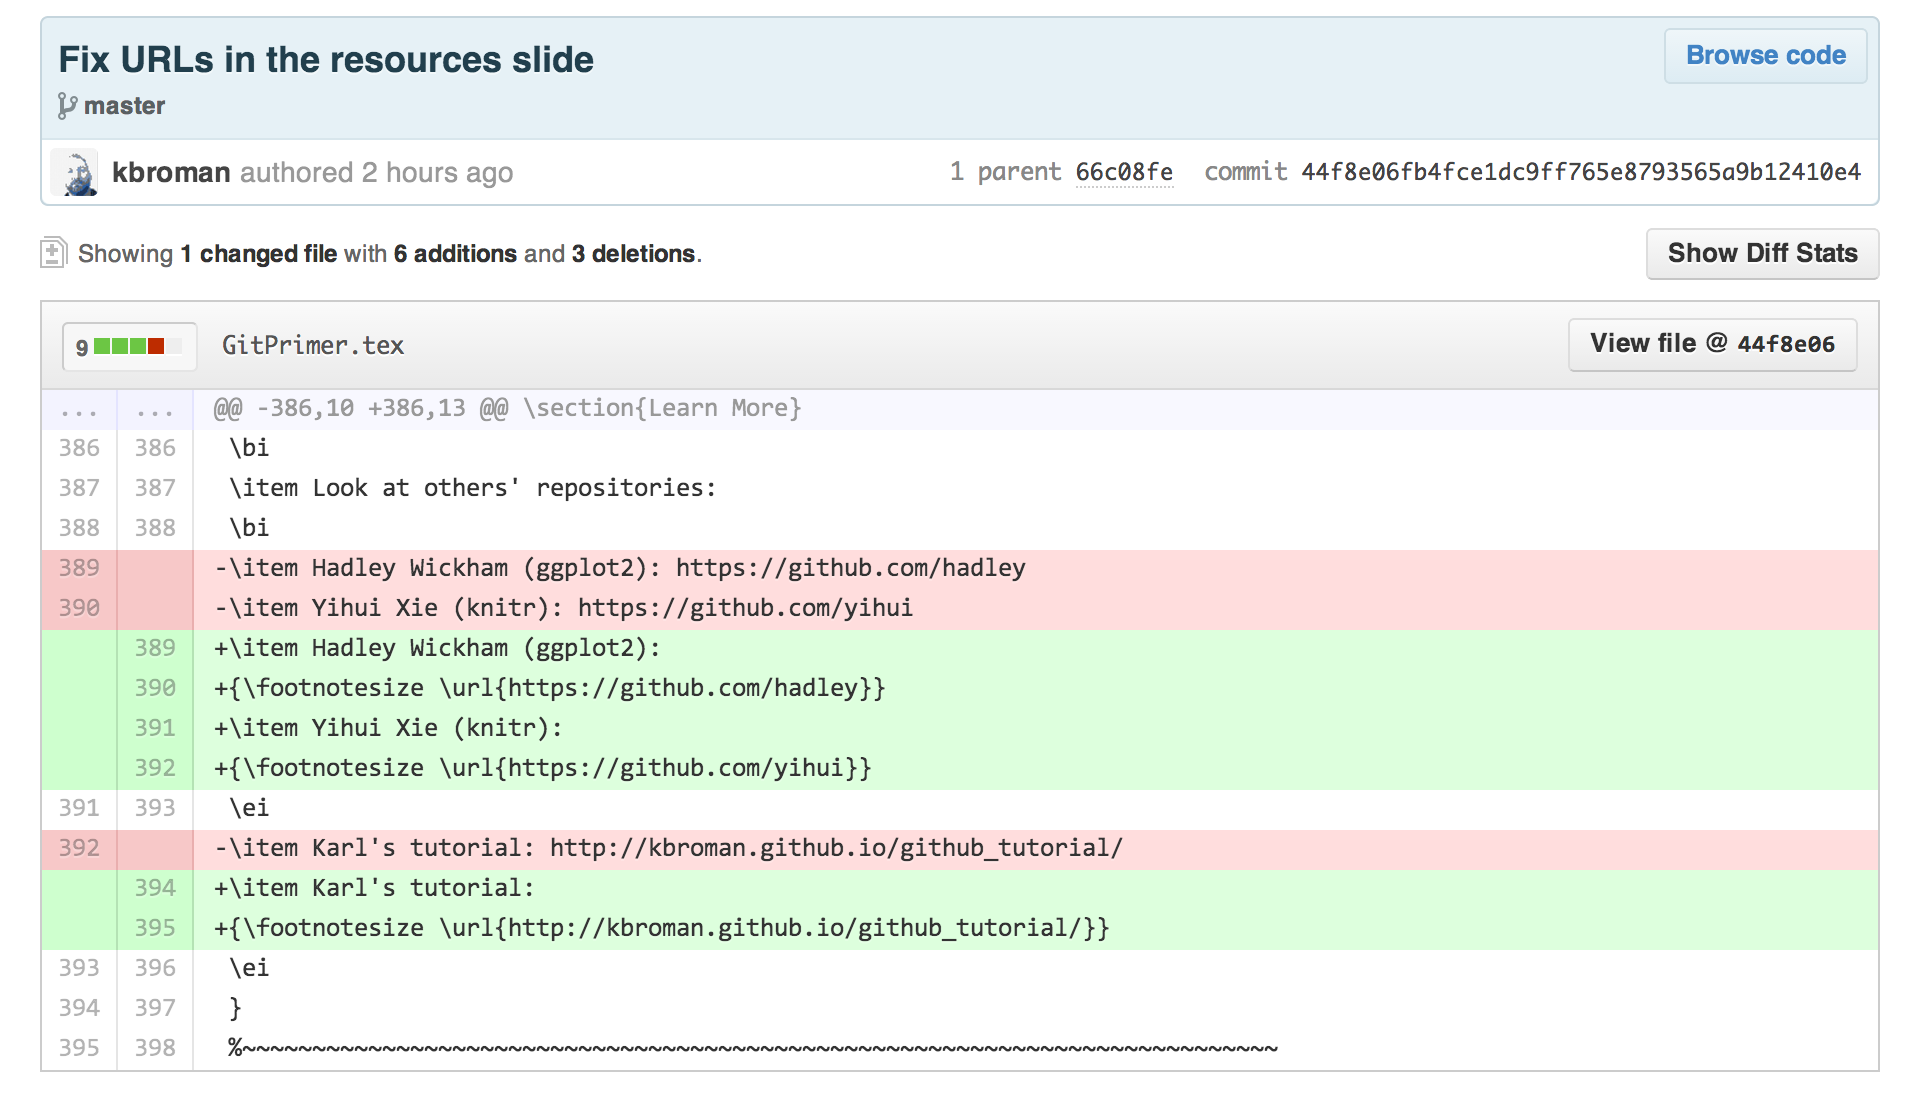
\includegraphics[height=2.2in]{a_commit.png}
\end{frame}


\begin{frame}[fragile]
\frametitle{Initialize}
\bbi
\item Create a working directory and initialize it to be a git
  repository
\ei
\begin{semiverbatim}
\begin{lstlisting}
$ mkdir ~/GitPrimer
$ cd ~/GitPrimer
$ git init
Initialized empty Git repository in ~/GitPrimer/.git/
\end{lstlisting}
\end{semiverbatim}
\end{frame}

\begin{frame}[fragile]
\frametitle{Produce Content}
\bbi
\item Create a README file

\begin{semiverbatim}
\begin{lstlisting}
Welcome to the GitPrimer repository.

Date: Tue Oct  1 14:12:47 CDT 2013

This repository contains source code for a brief git & GitHub tutorial
given by Younkin & Broman at the University of Wisconsin-Madison,
Dept. of Biostatistics & Medical Informatics.

Email Samuel Younkin <syounkin@stat.wisc.edu> with questions or
comments.
\end{lstlisting}
\end{semiverbatim}
\ei
\end{frame}

\begin{frame}[fragile]
\frametitle{Incorporate into Repository}
\bbi
\item Now we have the file README in our working directory, but it is not in the repository yet
\item We may check the status of the repository and working directory with \texttt{git status}
\ei
\begin{semiverbatim}
\begin{lstlisting}
$ git status
# On branch master
#
# Initial commit
#
# Untracked files:
#   (use "git add <file>..." to include in what will be committed)
#
#README
nothing added to commit but untracked files present (use "git add" to track)
\end{lstlisting}
\end{semiverbatim}

\end{frame}

\begin{frame}[fragile]
\frametitle{Incorporate into Repository}
\bbi
\item To include README in the repository we must first add README to the index using \texttt{git add}
\begin{semiverbatim}
\begin{lstlisting}
$ git add README 
\end{lstlisting}
\end{semiverbatim}
\ei
\end{frame}

\begin{frame}[fragile]
\frametitle{Incorporate into Repository}
\bbi
\item Now it is in the index, but it is not in the repository until it is "committed"
\bi
\item[] (it is "staged" for a commit)
\ei
\begin{semiverbatim}
\begin{lstlisting}
$ git status
# On branch master
#
# Initial commit
#
# Changes to be committed:
#   (use "git rm --cached <file>..." to unstage)
#
#new file:   README
\end{lstlisting}
\end{semiverbatim}
\ei
\end{frame}

\begin{frame}[fragile]
\frametitle{Incorporate into Repository}
\bbi
\item To commit to the repository we use \texttt{git commit}
\begin{semiverbatim}
\begin{lstlisting}
$ git commit -m "Initial commit of README file"
[master (root-commit) 32c9d01] Initial commit of README file
 1 file changed, 14 insertions(+)
 create mode 100644 README
\end{lstlisting}
\end{semiverbatim}
\item The \texttt{-m} argument allows one to enter a message in the command line
\item Without \texttt{-m}, \texttt{git} will spawn a text editor when you commit
\item git does not allow one to make a commit without entering a log message
\ei
\end{frame}

\begin{frame}[fragile]
\frametitle{Incorporate into Repository}
\bbi
\item Now that it has been committed it is in the repository 
\item We inspect the state of the repository again with \texttt{git log}
\ei
\begin{semiverbatim}
\begin{lstlisting}
$ git log
commit 32c9d013132948005408823e79216a891efe357c
Author: Samuel Younkin <syounkin@stat.wisc.edu>
Date:   Thu Oct 3 14:05:13 2013 -0500

    Initial commit of README file

\end{lstlisting}
\end{semiverbatim}
\end{frame}

\begin{frame}[fragile]
\frametitle{Incorporate into Repository}
\bbi
\item Let's look at the commit log for the repository as it was when I wrote this bullet point
{\footnotesize \begin{semiverbatim}
\begin{lstlisting}
$ git log --pretty=format:"%h - %an, %ar : %s" -10
e946257 - Samuel Younkin, 26 minutes ago : Added *.vrb to .gitignore
9c2b943 - Samuel Younkin, 22 hours ago : Worked on first four sections
311a538 - Karl Broman, 2 days ago : chmod on GitPrimer.tex (not executable)
516108b - Karl Broman, 2 days ago : Add a Makefile
b7fbf7b - Karl Broman, 2 days ago : Remove the Thank you page
c072fbc - Karl Broman, 2 days ago : Simplify institution and split into two lines
173091b - Samuel Younkin, 2 days ago : Fixed time-stamping in README
92a585c - Samuel Younkin, 2 days ago : Initial commit
\end{lstlisting}
\end{semiverbatim}}
\item We include arguments to \texttt{git log} to make the output more readable.
\ei
\end{frame}


\frame{
\ft{A few points on commits}
\bbi
\item Use frequent, small commits
\item Don't get out of sync with your collaborators
\item Commit the sources, not the derived files
\bi
\item[] (R code not images)
\ei
\ei
}


\section{GitHub}

\frame{
\ft{What is GitHub?}
\bbi
\item Like facebook for programmers
\item A home for git repositories
\item Interface for exploring git repositories
\item (Bitbucket.org is an alternative)
\ei
}

\frame{
\ft{Why use GitHub?}
\bbi
\item It takes care of the server aspects of git
\item Facilitates:
\bi
\item Learning from others
\item Seeing what people are up to
\item Contributing to others' code
\ei
\item Lowers the barrier to collaboration
\ei
}

\section{GitHub Demo}

\frame{
\ft{Getting started with GitHub}
\bbi
\item Get an account
\item Set up ssh keys
\item Create a new repository
\ei
}

\frame{
\ft{Fork, clone, push, \& pull}
\bbi
\item Fork someone's repository
\item Clone your version of it
\item Change things locally
\item Push your changes
\ei
}

\frame{
\ft{Issues and pull requests}
\bbi
\item Problem with or suggestion for someone's code?
\bi
\item Point it out as an Issue
\ei
\item Even better: Provide a fix
\bi
\item Fork
\item Clone
\item Modify
\item Push
\item Submit a Pull Request
\ei
\ei
}


\section{Learn More}
\frame{
\ft{Resources}
\bbi
\item Look at others' repositories:
\bi
\item Hadley Wickham (ggplot2):
{\footnotesize \url{https://github.com/hadley}}
\item Yihui Xie (knitr):
{\footnotesize \url{https://github.com/yihui}}
\ei
\item Karl's tutorial:
{\footnotesize \url{http://kbroman.github.io/github_tutorial/}}
\ei
}

\end{document}
